\chapter{Badanie układów TTL}

\section{Układ 7400 (NAND)}

\begin{itemize}
    \item Schemat pinów dla układu \textbf{TTL 7400} (NAND):
        \begin{figure}[H]
            \centering
            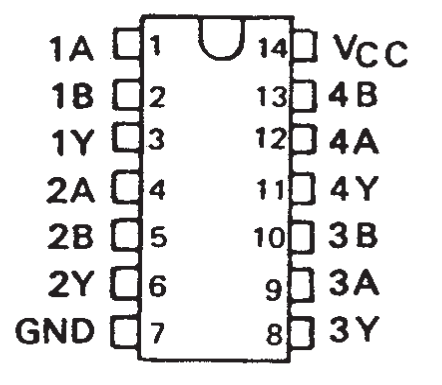
\includegraphics[scale=0.25]{img/schemes/NAND_7400_pins.png}
            \caption{Piny 7400 (NAND)}
            \label{NAND:piny}
        \end{figure}
    \item Według schematu w układzie znajdują się: 
        \begin{center}
            pin uziemiający (\textbf{GND}) - pin \textbf{7} \\
            pin zasilający (\textbf{VCC}) - pin \textbf{14} \\
            piny wejścia (\textbf{iA}, \textbf{iB}) \\
            piny wyjścia (\textbf{iY}) \\
            \textbf{gdzie i - numer bramki logicznej}
        \end{center}
    \item Podpięto zasilanie oraz uziemienie. Podpinając wyjście z \textbf{1} impulsatora (wyższego) do \textbf{pinu 1}, a wyjście z \textbf{2} impulsatora do \textbf{pinu 2} oraz wyjście (\textbf{pin 3}) do próbnika stanów logicznych przetestowano bramkę NAND.
        \begin{figure}[H]
            \centering
                \begin{subfigure}[h]{0.4\textwidth}
                    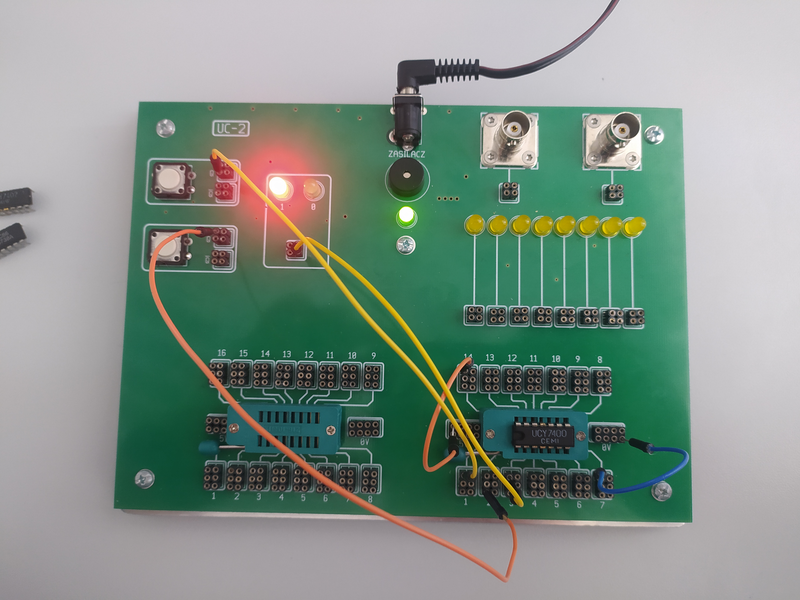
\includegraphics[width=\textwidth]{img/NAND/test/1652306732892_scaled.png}
                \end{subfigure}
                \begin{subfigure}[h]{0.4\textwidth}
                    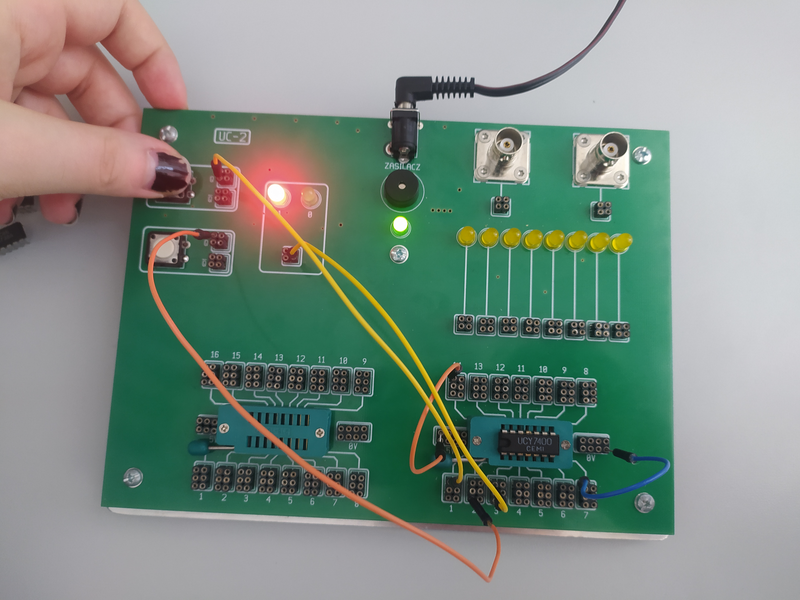
\includegraphics[width=\textwidth]{img/NAND/test/1652306732884_scaled.png}
                \end{subfigure}
                \begin{subfigure}[h]{0.4\textwidth}
                    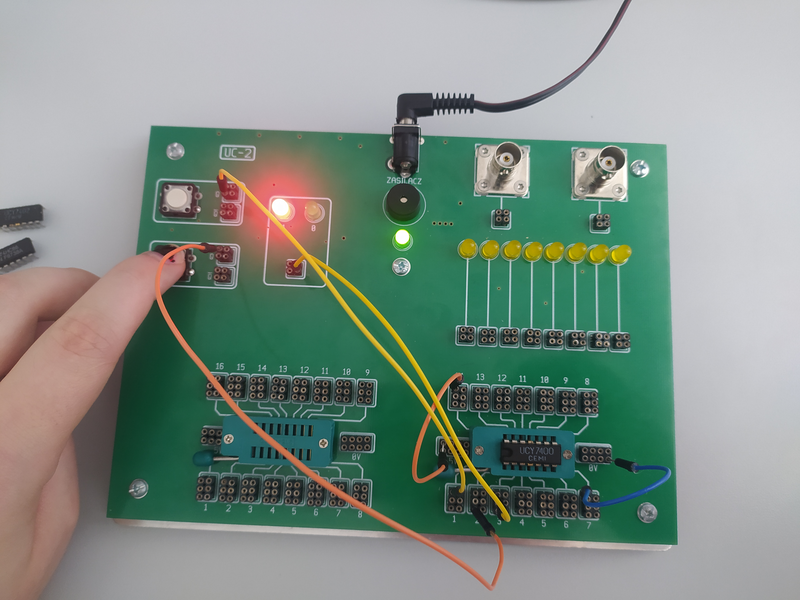
\includegraphics[width=\textwidth]{img/NAND/test/1652306732872_scaled.png}
                \end{subfigure}
                \begin{subfigure}[h]{0.4\textwidth}
                    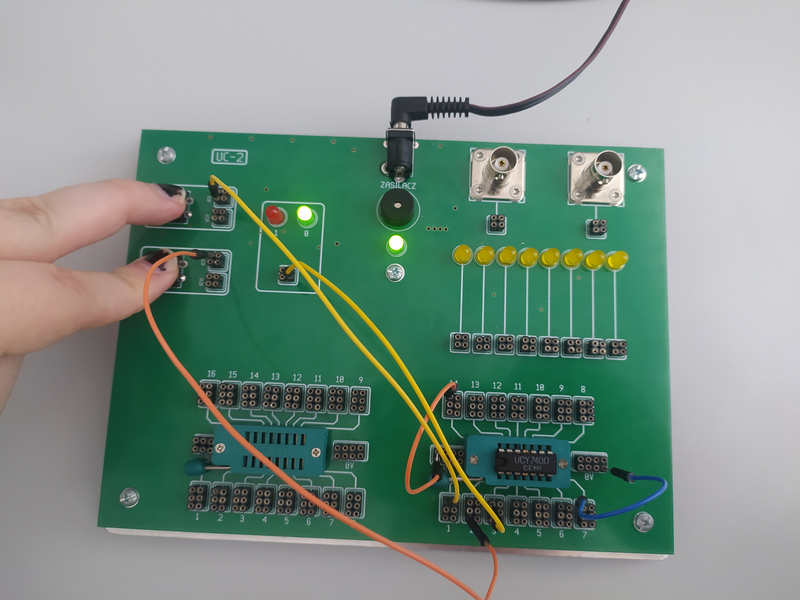
\includegraphics[width=\textwidth]{img/NAND/test/1652306732862_scaled.png}
                \end{subfigure}
        \end{figure}

\pagebreak

    \item Tabela stanów wyznaczona doświadczalnie:
        \begin{center}
            \begin{tabular}{|c|c|>{\columncolor[gray]{0.8}}c|}
                \hline
                A & B & Y \\
                \hline
                0 & 0 & 1 \\
                \hline
                0 & 1 & 1 \\
                \hline
                1 & 0 & 1 \\
                \hline
                1 & 1 & 0 \\
                \hline
            \end{tabular}
        \end{center}
    \item Napięcia wyjściowe dla logicznych 0 (L) oraz 1 (H):
        \begin{figure}[H]
            \centering
                \begin{subfigure}[h]{0.49\textwidth}
                    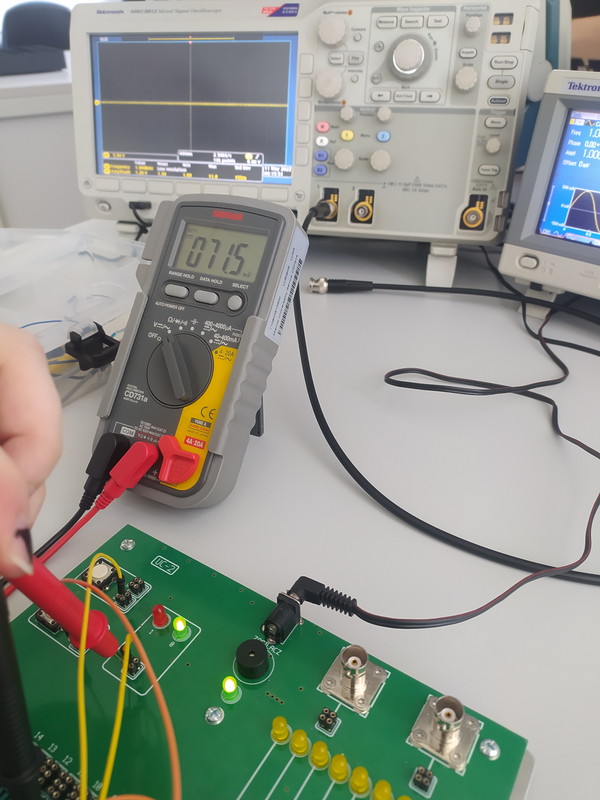
\includegraphics[width=\textwidth]{img/NAND/test/1652306732837_scaled.png}
                    \caption*{Pomiar dla L}
                \end{subfigure}
                \begin{subfigure}[h]{0.49\textwidth}
                    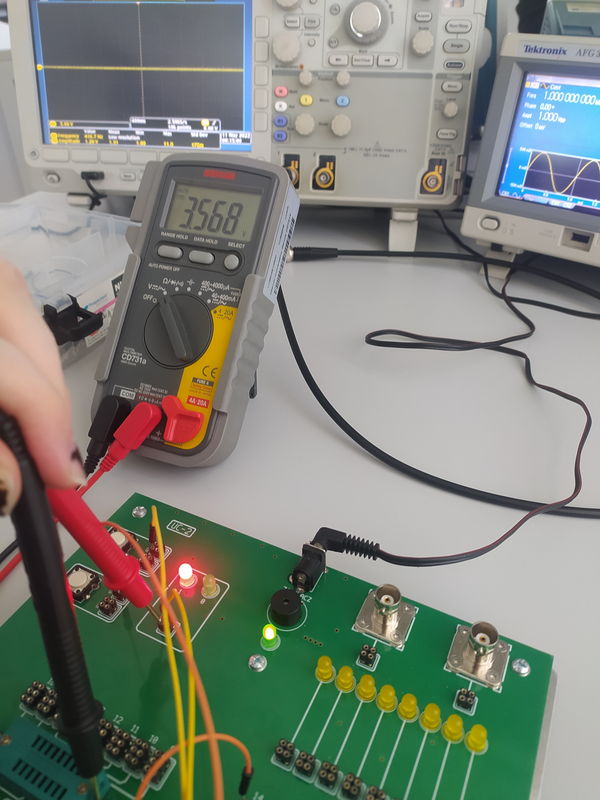
\includegraphics[width=\textwidth]{img/NAND/test/1652306732851_scaled.png}
                    \caption*{Pomiar dla H}
                \end{subfigure}
            \label{płytka:pomiar_impulsatorów}
        \end{figure}
        \begin{gather}
            U_{low} = \textbf{0.071V} \\
            U_{high} = \textbf{3.568V}
        \end{gather}
    \item Napięcia zgadzają się ze standardem TTL (\autoref{TTL:charakterystyka}).
\end{itemize}

\pagebreak

\section{Układ 7402 (NOR)}

\begin{itemize}
    \item Schemat pinów dla układu \textbf{TTL 7402} (NOR):
        \begin{figure}[H]
            \centering
            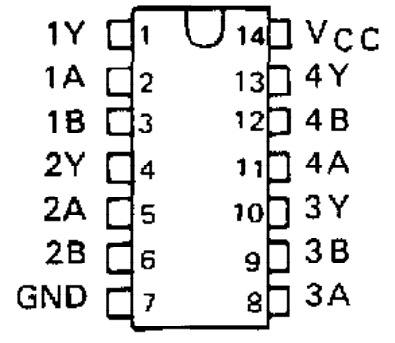
\includegraphics[scale=0.25]{img/schemes/NOR_7402_pins.png}
            \caption{Piny 7402 (NOR)}
            \label{NOR:piny}
        \end{figure}
    \item Według schematu w układzie znajdują się: 
        \begin{center}
            pin uziemiający (\textbf{GND}) - pin \textbf{7} \\
            pin zasilający (\textbf{VCC}) - pin \textbf{14} \\
            piny wejścia (\textbf{iA}, \textbf{iB}) \\
            piny wyjścia (\textbf{iY}) \\
            \textbf{gdzie i - numer bramki logicznej}
        \end{center}
    \item W odróżnieniu od schematu dla układu NAND (\ref{NAND:piny}) wyjścia z impulsatorów podpięto do pinów \textbf{2},\textbf{3}, zaś wyjście (\textbf{pin 1}) do próbnika stanów logicznych.
        \begin{figure}[H]
            \centering
                \begin{subfigure}[h]{0.4\textwidth}
                    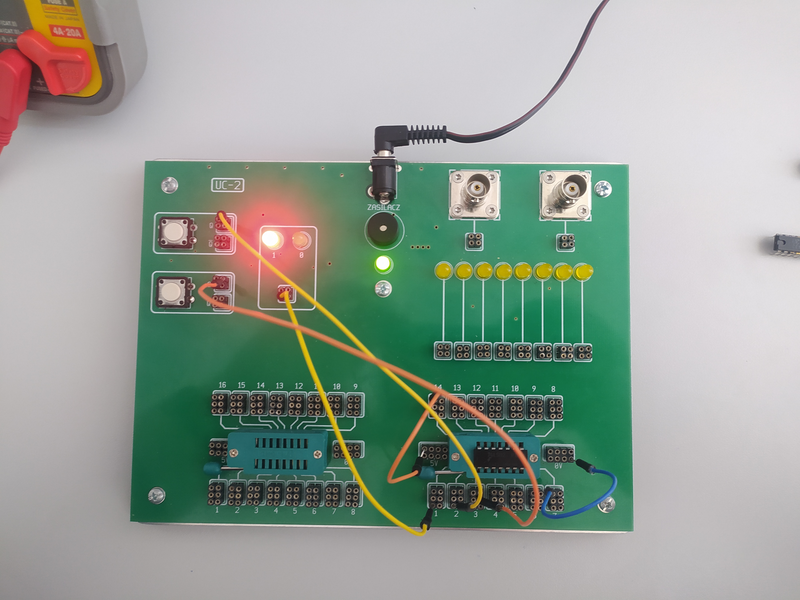
\includegraphics[width=\textwidth]{img/NOR/test/1652306732823_scaled.png}
                \end{subfigure}
                \begin{subfigure}[h]{0.4\textwidth}
                    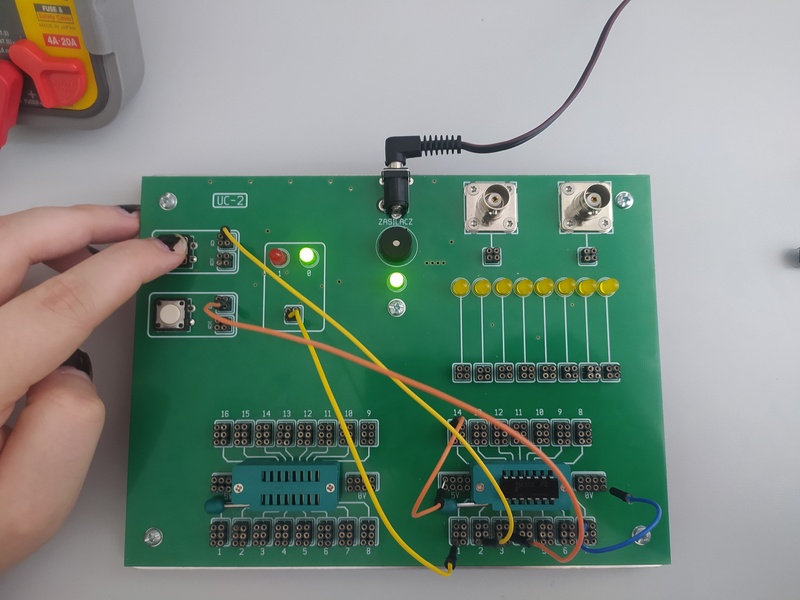
\includegraphics[width=\textwidth]{img/NOR/test/1652306732810_scaled.png}
                \end{subfigure}
                \begin{subfigure}[h]{0.4\textwidth}
                    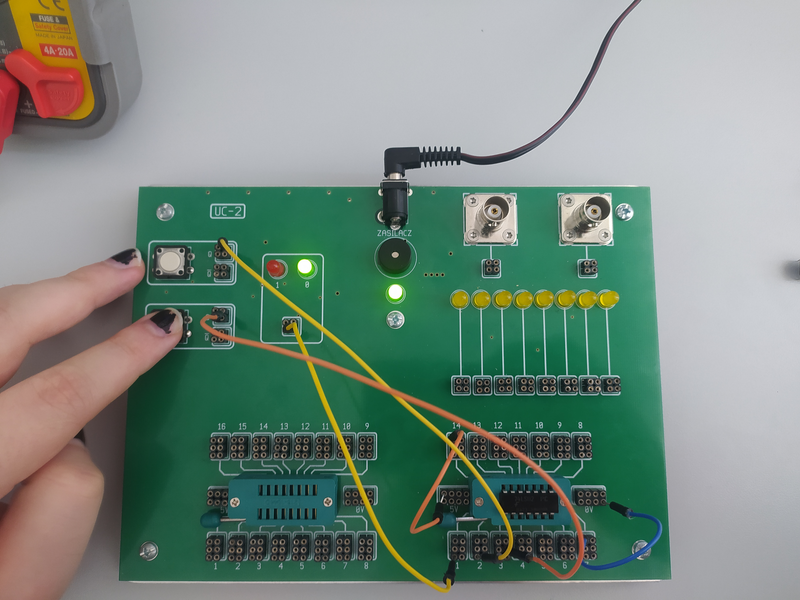
\includegraphics[width=\textwidth]{img/NOR/test/1652306732798_scaled.png}
                \end{subfigure}
                \begin{subfigure}[h]{0.4\textwidth}
                    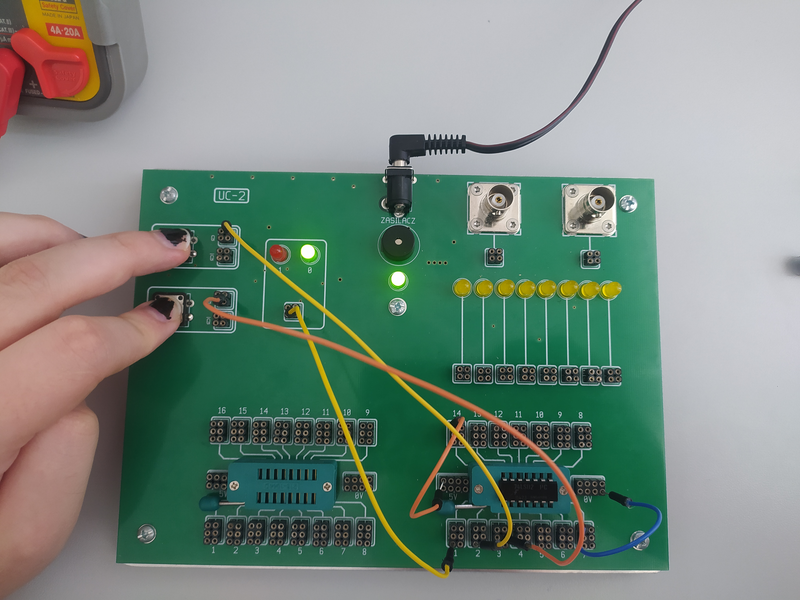
\includegraphics[width=\textwidth]{img/NOR/test/1652306732785_scaled.png}
                \end{subfigure}
        \end{figure}

\pagebreak

    \item Tabela stanów wyznaczona doświadczalnie:
        \begin{center}
            \begin{tabular}{|c|c|>{\columncolor[gray]{0.8}}c|}
                \hline
                A & B & Y \\
                \hline
                0 & 0 & 1 \\
                \hline
                0 & 1 & 0 \\
                \hline
                1 & 0 & 0 \\
                \hline
                1 & 1 & 0 \\
                \hline
            \end{tabular}
        \end{center}
    \item Napięcia wyjściowe dla logicznych 0 (L) oraz 1 (H):
        \begin{figure}[H]
            \centering
                \begin{subfigure}[h]{0.49\textwidth}
                    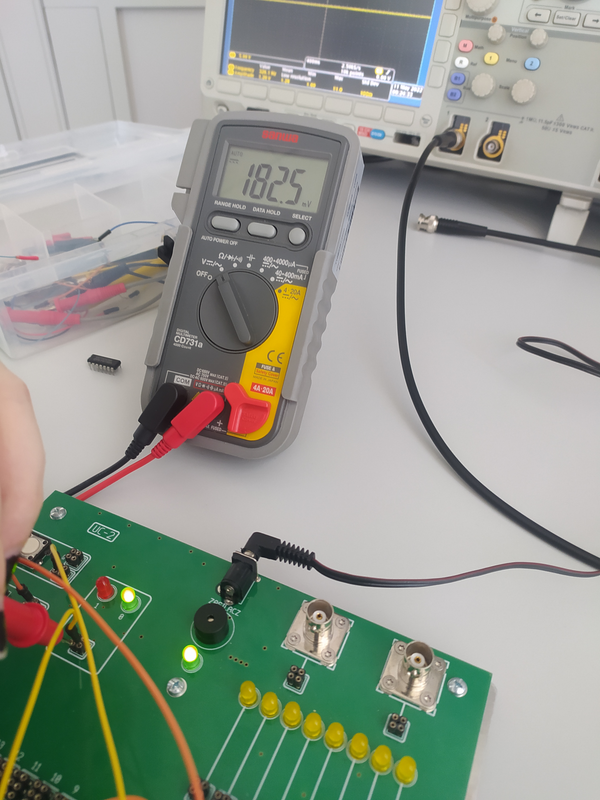
\includegraphics[width=\textwidth]{img/NOR/test/1652306732756_scaled.png}
                    \caption*{Pomiar dla L}
                \end{subfigure}
                \begin{subfigure}[h]{0.49\textwidth}
                    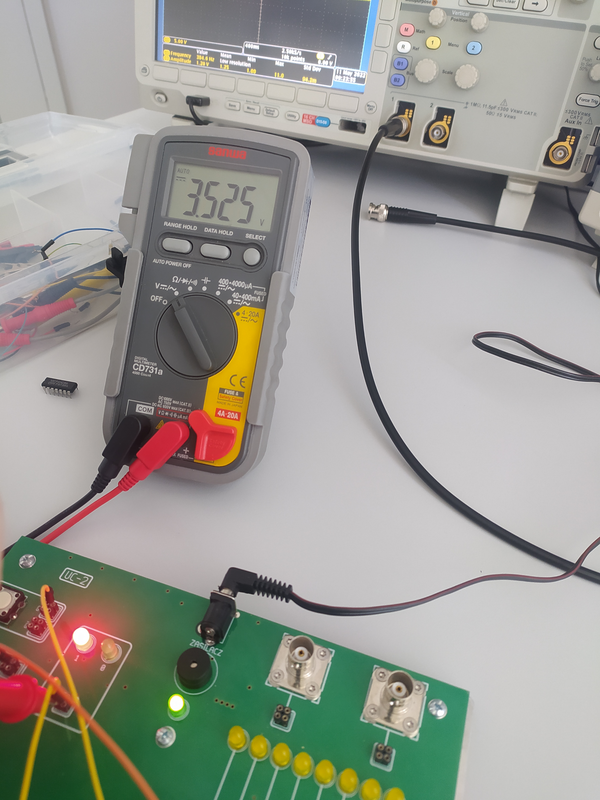
\includegraphics[width=\textwidth]{img/NOR/test/1652306732772_scaled.png}
                    \caption*{Pomiar dla H}
                \end{subfigure}
            \label{płytka:pomiar_impulsatorów}
        \end{figure}
        \begin{gather}
            U_{low} = \textbf{0.182V} \\
            U_{high} = \textbf{3.525V}
        \end{gather}
    \item Napięcia zgadzają się ze standardem TTL (\autoref{TTL:charakterystyka}).
\end{itemize}

\pagebreak

\section{Układ 7486 (XOR)}

\begin{itemize}
    \item Schemat pinów dla układu \textbf{TTL MC74HC86} (XOR):
        \begin{figure}[H]
            \centering
            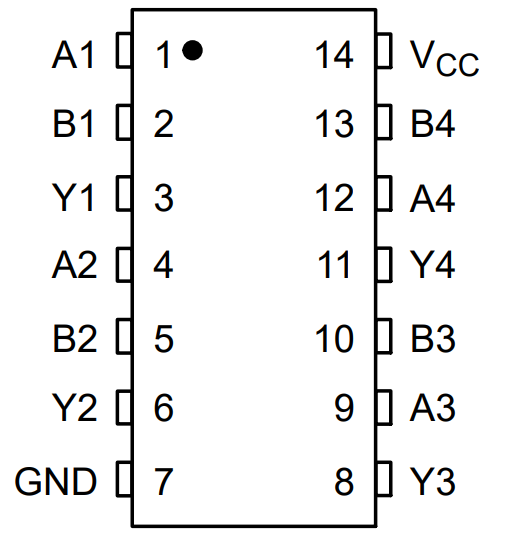
\includegraphics[scale=0.25]{img/schemes/XOR_mc74hc86_pins.png}
            \caption{Piny 7486 (XOR)}
            \label{XOR:piny}
        \end{figure}
    \item Według schematu w układzie znajdują się: 
        \begin{center}
            pin uziemiający (\textbf{GND}) - pin \textbf{7} \\
            pin zasilający (\textbf{VCC}) - pin \textbf{14} \\
            piny wejścia (\textbf{iA}, \textbf{iB}) \\
            piny wyjścia (\textbf{iY}) \\
            \textbf{gdzie i - numer bramki logicznej}
        \end{center}
    \item Piny wejściowe oraz wyjściowe ułożone \textbf{są tak samo jak} dla schematu dla układu \textbf{NAND} (\ref{NAND:piny}) wyjścia z impulsatorów podpięto do pinów 1,2, zaś wyjście (pin 3) do próbnika stanów logicznych.
        \begin{figure}[H]
            \centering
                \begin{subfigure}[h]{0.4\textwidth}
                    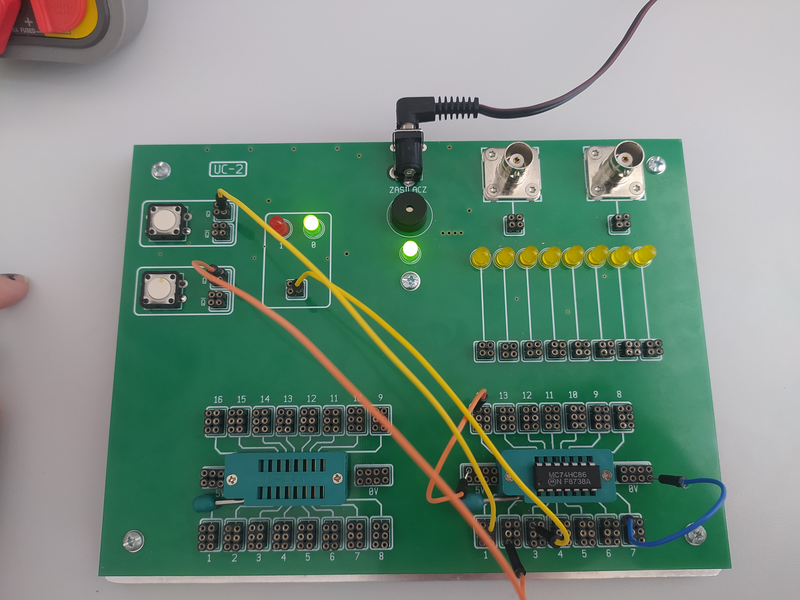
\includegraphics[width=\textwidth]{img/XOR/test/1652306732731_scaled.png}
                \end{subfigure}
                \begin{subfigure}[h]{0.4\textwidth}
                    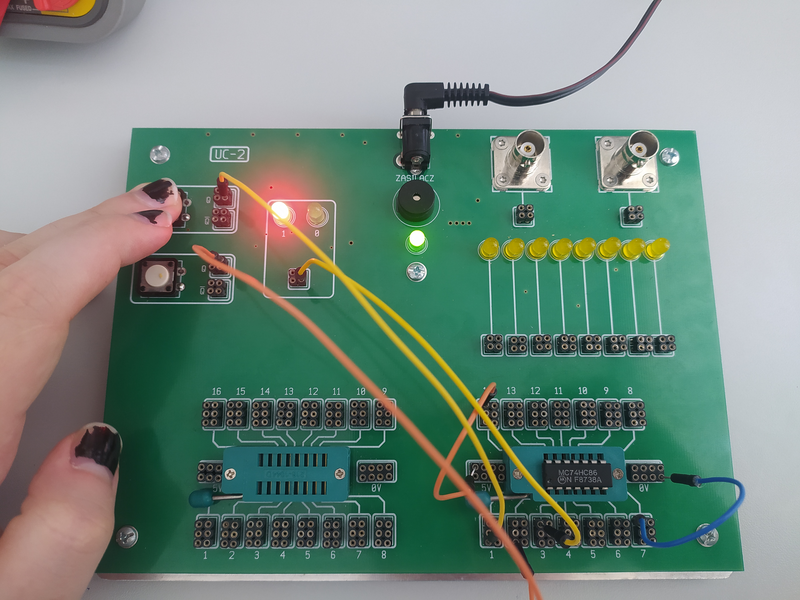
\includegraphics[width=\textwidth]{img/XOR/test/1652306732718_scaled.png}
                \end{subfigure}
                \begin{subfigure}[h]{0.4\textwidth}
                    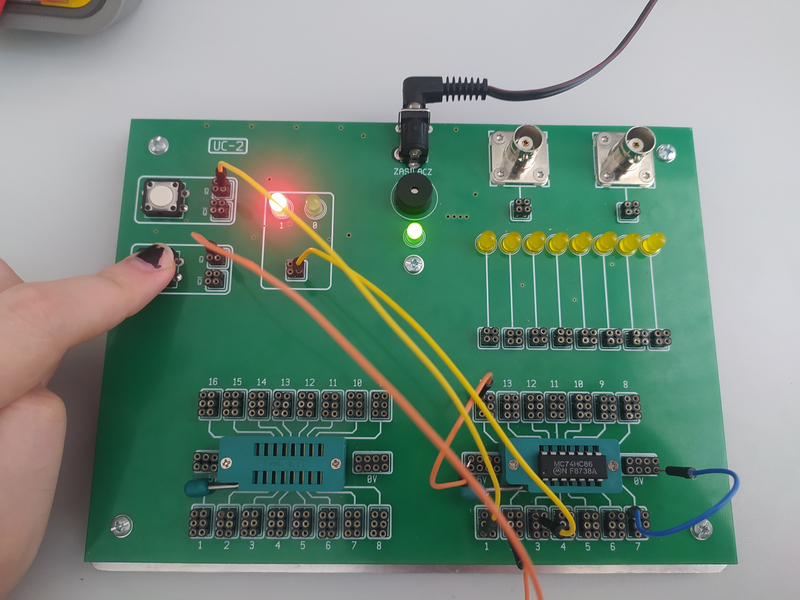
\includegraphics[width=\textwidth]{img/XOR/test/1652306732707_scaled.png}
                \end{subfigure}
                \begin{subfigure}[h]{0.4\textwidth}
                    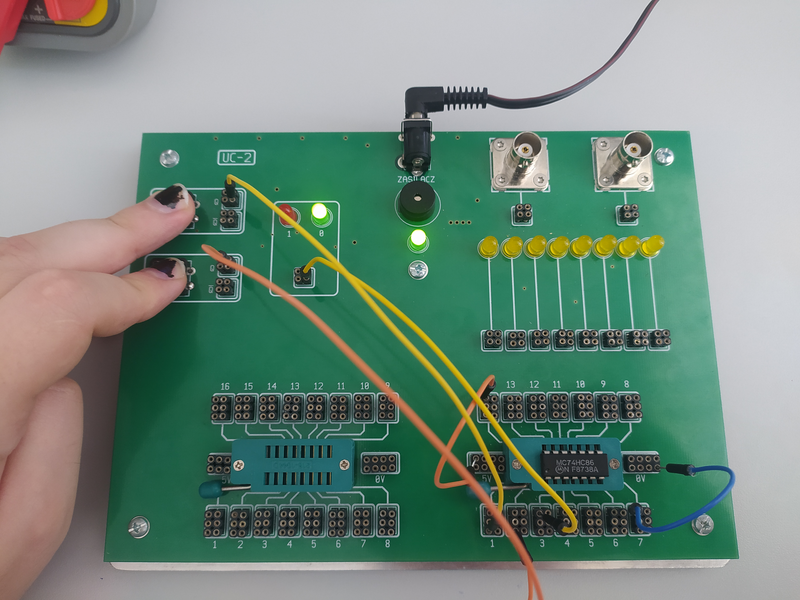
\includegraphics[width=\textwidth]{img/XOR/test/1652306732690_scaled.png}
                \end{subfigure}
        \end{figure}

\pagebreak

    \item Tabela stanów wyznaczona doświadczalnie:
        \begin{center}
            \begin{tabular}{|c|c|>{\columncolor[gray]{0.8}}c|}
                \hline
                A & B & Y \\
                \hline
                0 & 0 & 1 \\
                \hline
                0 & 1 & 0 \\
                \hline
                1 & 0 & 0 \\
                \hline
                1 & 1 & 0 \\
                \hline
            \end{tabular}
        \end{center}
    \item Napięcia wyjściowe dla logicznych 0 (L) oraz 1 (H):
        \begin{figure}[H]
            \centering
                \begin{subfigure}[h]{0.4\textwidth}
                    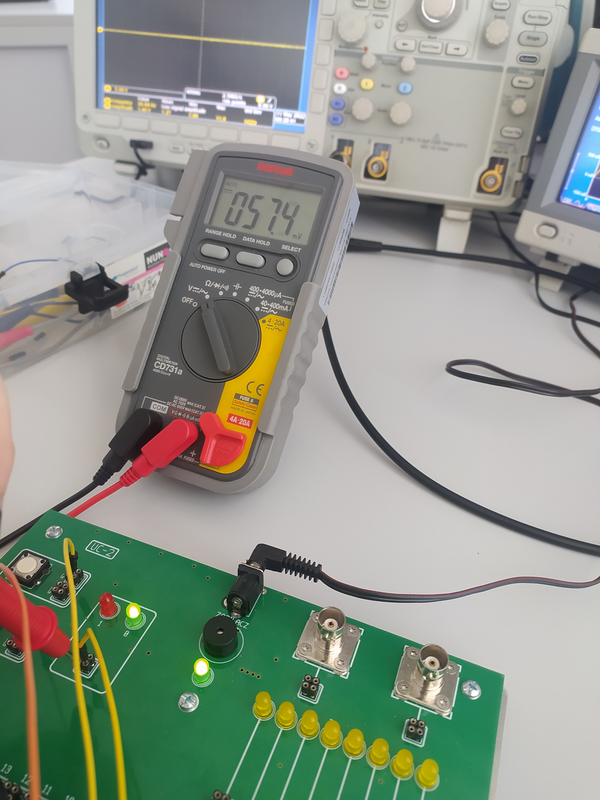
\includegraphics[width=\textwidth]{img/XOR/test/1652306732674_scaled.png}
                    \caption*{Pomiar dla L}
                \end{subfigure}
                \begin{subfigure}[h]{0.4\textwidth}
                    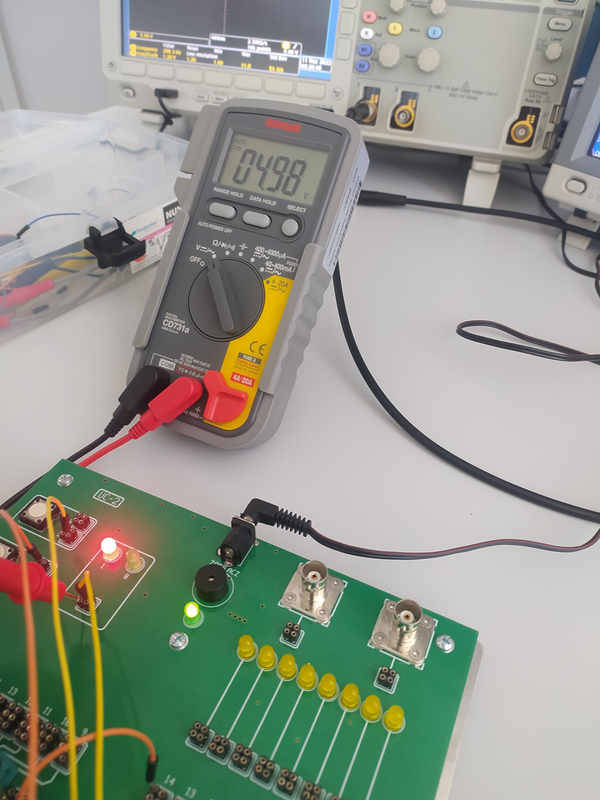
\includegraphics[width=\textwidth]{img/XOR/test/1652306732649_scaled.png}
                    \caption*{Pomiar dla H}
                \end{subfigure}
            \label{płytka:pomiar_impulsatorów}
        \end{figure}
        \begin{gather}
            U_{low} = \textbf{0.057V} \\
            U_{high} = \textbf{4.98V}
        \end{gather}
    \item Napięcia zgadzają się ze standardem TTL (\autoref{TTL:charakterystyka}).
\end{itemize}